\section{Winner-Take-All networks}

It has been discovered that pyramidal neurons on layers 2/3 and 5/6 of the neocortex form selection networks. This means that one pyramidal neuron is allowed to fire, while others within the same layer are inhibited. This horizontal selection mechanism determines what is vertically sent on to the neurons of cortical layers higher up in the hierarchy. For example pyramidal neurons in layer 5 have a selection behaviour that determines the output to motor structures. Their inhibition is performed by basket and chandelier cells \citep{softWTA}. Basket cells connect to the soma of other neurons and control the action potential discharge rate of those neurons. Their dendritic branches wrap around the target soma, forming a "basket" giving them their name \citep{basketCells}. Chandelier cells perform inhibition directly at the axonal initial segment of pyramidal neurons where action potentials are initiated. \citep{chandelierCells}. The selection of one pyramidal neuron performed this way is called soft winner-take-all mechanism and is used in various neuronal network models \citep{softWTA}. The mechanism is called "soft" because it uses a softmax function, which controls how many winners there can be, and how likely each neuron is to win \citep{handbookWTA}. It has been shown that winner-take-all mechanisms are computationally more powerful when compared to threshold gates (McCulloch-Pitts neurons) and sigmoidal gates. Furthermore, arbitrary continuous functions can be approximated by circuits that only include one soft winner-take-all gate as their only nonlinear operator \citep{WTAPower}.

\section{The hierarchical structure of the brain}

The brain is made up of modular structures that connect with each other in a hierarchical organization. These modules have a high level of connectivity within themselves and a low level to other modules. This means that there are different categories of neurons within a module, depending on their function in the network. For one there are provincial hub neurons that primarily connect to other neurons of the same module and are responsible for the function the module expresses. Then there are connector hub neurons that transfer information from the module to other modules. Such modules form networks which are connected in a hierarchical manner, where each module is adding to the output of the previous module \citep{hierarchicalBrain}.
Most of the information flows upwards along the hierarchy, representing bottom-up observations. But there is physiological experimental data that shows that information is also passed downwards and influences the activity of modules lower in the hierarchy, representing top-down context. This will be explained for the visual cortex.

\section{Visual cortex}

The visual cortex is the region of the brain that processes visual information coming from the retina. From the retina the information is sent to the lateral geniculate nucleus in the thalamus and then further to the primary visual cortex, also called visual area 1 (V1). The visual cortex consists of five visual areas (V1 to V5), which are divided by their function and structure. These areas are located in the occipital lobe of the cerebral cortex. The purpose of the visual areas is to process visual information to recognize objects, perform spatial tasks or to perform  visual-motor skills. Neurons of the visual cortex often respond to stimuli within a specific receptive field. It is assumed that each subsequent visual area is more specialized than the previous and due to that neurons in different visual areas respond to the same receptive fields, but to different types of stimuli. There are various specialized cells in the visual cortex. For example simple cells and complex cells are well studied. Simple cells which mainly occur in V1 respond primarily to oriented edges and lines within a receptive field. For example a simple cell would always generate action potentials when there is a horizontal line in its receptive field. Complex cells can be found in V1, V2 and V3 and also respond primarily to oriented edges and lines. However their receptive fields are larger and an horizontal edge for example does not have to be at a specific location in the receptive field to activate the cell. Some complex cells even respond primarily to movement of edges \citep{visualCortexBook}.
This activation of neurons depending on the stimulus is called neuronal tuning. The stimuli the complex cells respond to get more complex, the higher up in the visual cortex hierarchy they are located. For example in the inferior temporal cortex, which receives visual information from V4, there are complex cells that respond to faces \citep{complexCellsFaces}.
According to \citet{complexCellsIntegrated} the larger receptive fields of complex cells are due to the hierarchical convergent nature of visual processing. This property follows from the complex cell receiving input from many simple cells which is summed and integrated.

Visual information first enters V1, which is the best-understood part of the visual cortex. It consists of six layers that function differently. Layer 4 receives the input from the lateral geniculate nucleus. It has the most simple cells of the six layers and thus processes visual information of small receptive fields. On layers 2, 3 and 6 there are complex cells, which combine the result of layer 4 into larger receptive fields. Through that V1 outputs simple visual components with their orientation or direction. The processed information is then sent on to V2 which further processes it and thus responds to more visual complex patterns. V2 was also found to respond to differences in color and spatial frequency, additional to the more complex patterns and object orientation. After processing V2 sends its information on to V3, V4 and V5. Furthermore it also has feedback connections to V1, which will be discussed later. After V2 the visual information is split up into the dorsal and ventral streams, which each specialize in processing different features of the visual information. The dorsal stream is involved in guidance of motor actions and in recognizing where objects are in space. The ventral stream on the other hand is responsible for object recognition and form representation.
\citep{visualCortexBook}

\section{Probabilistic brain}

\citet{probabilisticBrain} state that there is strong behavioural and physiological evidence that the brain both represents probability distributions and performs probabilistic inference. Because of that there are several experiments that support a mathematical framework based on Bayesian inference (see Chapter \ref{section:bayesianInference}) to model brain computations. \citep{neuralSubstrate, HierachicalBayesVisualCortex, anatomyOfInference, neuralImplementationOfBayesionInferenceSensoryMotor}. An advantage of these probabilistic models is their generality, meaning that they can be applied to various tasks that the brain performs \citep{probabilisticBrain}. 
TODO!!!!!
1. What is the connection to your work?	

\section{Feedback in the visual cortex}
\label{section:feedbackInVisualCortex}
\citet{HierachicalBayesVisualCortex} showed that feedback in the visual cortex is not only used for attentional selection or biased competition, but also to modulate the processing of the early visual cortex. Furthermore they showed how this modulated processing can be explained via hierarchical Bayesian inference. One hypothetical example for the modulation of lower hierarchical areas that they give is a human looking at a picture of a face which is partially in shadow. First V1 receives the information of the image and performs edge and line detection. In this initial processing the detected edges are in the well lit portion of the image, while in the shadowy part almost no edges are found. As this information is passed on upwards along the visual cortex hierarchy it is processed further, until it reaches the inferior temporal cortex where the conclusion is made that there is a face in the picture. After that, feedback is sent from the inferior temporal cortex back to V1. This feedback tells V1 that there should be edges hidden in the shadow. With this additional prior information V1 then is able to detect the faint edge in the shadow and complete the contour of the face. 
In one of their experiments they made a monkey look at a fixation spot on a screen while Kanizsa squares were presented one at a time in different locations. Kanizsa squares are optical illusions where an illusory square can be seen between four partial disks. One such image can be seen in Figure \ref{fig:KanizsaSquare}. The illusory square is seen because the brain chooses the simplest interpretation that a white square is lying on top of the black circles, occluding them.
\begin{figure}
  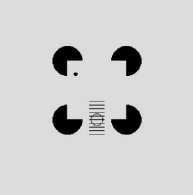
\includegraphics[width=\linewidth]{figures/kanizsaSquare.PNG}
  \caption{Kanizsa square shown to the monkey by \citet{HierachicalBayesVisualCortex}}
  \label{fig:KanizsaSquare}
\end{figure}
During the presentation neuronal activity in V1 and V2 was measured. When looking at a single neuron in V1, which has a receptive field size of less than 0.8 degrees, they reported that it responds with increased spiking activity within 45 ms after a real line appears in its receptive field. When that neuron has an illusory line of the Kanizsa square in its receptive field it is not active within 45 ms. However after 100 ms it begins to respond, indicating that it starts seeing the illusory line. In contrast, the measured population of 39 V2 neurons responded to the illusory contour after 65 ms, 35 ms before V1. They explained this behaviour as V2 detecting the illusory contour with information from a spatially more global context and then feeding back that information (prior) to V1. V1 then, convinced by V2, starts hallucinating the illusory line, agreeing with the most likely interpretation of the image. This experiment provides strong evidence that feedback is happening in the hierarchical structure of the visual cortex.

\section{Plasticity}
TODO!!!!
first reading SpikingNeuronModelsBook...
ES IST PERFEKT PDF Seite 99!!

\section{Spiking neural networks}

Spiking neural networks (SNNs) are artificial neural networks that resemble biological neural networks more closely. Neurons in typical neural networks used in machine learning transmit information at every propagation cycle. This, however, is not how biological neurons operate. They generate action potentials (neuron spikes) to convey information between each other. These action potentials are only generated when their membrane potential exceeds a threshold. SNN models take this behaviour into account by keeping track of each neurons membrane potential and then determining when they should produce an action potential  \citep{SpikingNeuronModelsBook}.

Previously it was believed that biological neural networks encode information within the spike rates of neurons. However neurobiological research shows evidence that at high speed processing this alone can not be sufficient. For example image recognition tasks can be performed at a speed at which each neuron in the involved layers has only less than 10 ms to process the information. Such a time frame is too short for rate coding to occur. Instead it has been shown that high speed processing tasks can be performed using the precise timing of spikes. Furthermore it requires more energy for a neuron to spike many times to express a spike rate, rather than spiking just once and having the timing of the spike considered. As the brain evolutionarily aims to minimize its energy consumption this is a strong argument for spike timing encoded information. Also the information encoding capacity is higher in a small set of spiking neurons, compared to rate encoding. \citep{LearningInBiologicallyPlausibleSNN}
Because of that Spike Timing Dependent Plasticity (STDP) is often used as learning rule in SNNs. STDP models the synaptic weight changes of neurons depending on the relative timing of pre- and postsynaptic spikes. If a presynaptic spike arrives shortly before the postsynaptic spike the synaptic weight is increased. The size of that increase depends exponentially on the time between both spikes, according to a time constant. However, when the presynaptic spike occurs after the postsynaptic spike the synaptic weight is decreased. These two mechanisms are called long-term potentiation and long-term depression respectively. Although STDP is often modelled like this, biological experiments show that the standard pair-based approach does not fully explain it in biological neurons. However, there is experimental evidence that multiple-spike protocols like triplets STDP are biologically more plausible. 
\citep{LearningInBiologicallyPlausibleSNN}	